% Copyright (C) 2015 Glen Newton
% Author: Glen Newton
%  Licensed under a Creative Commons Attribution-NonCommercial-ShareAlike 4.0 International License

\documentclass{article}
\usepackage{tikz}
\usetikzlibrary{shapes.geometric,arrows,positioning}
%\usepackage{helvet}

\renewcommand{\familydefault}{\sfdefault}

\begin{document}
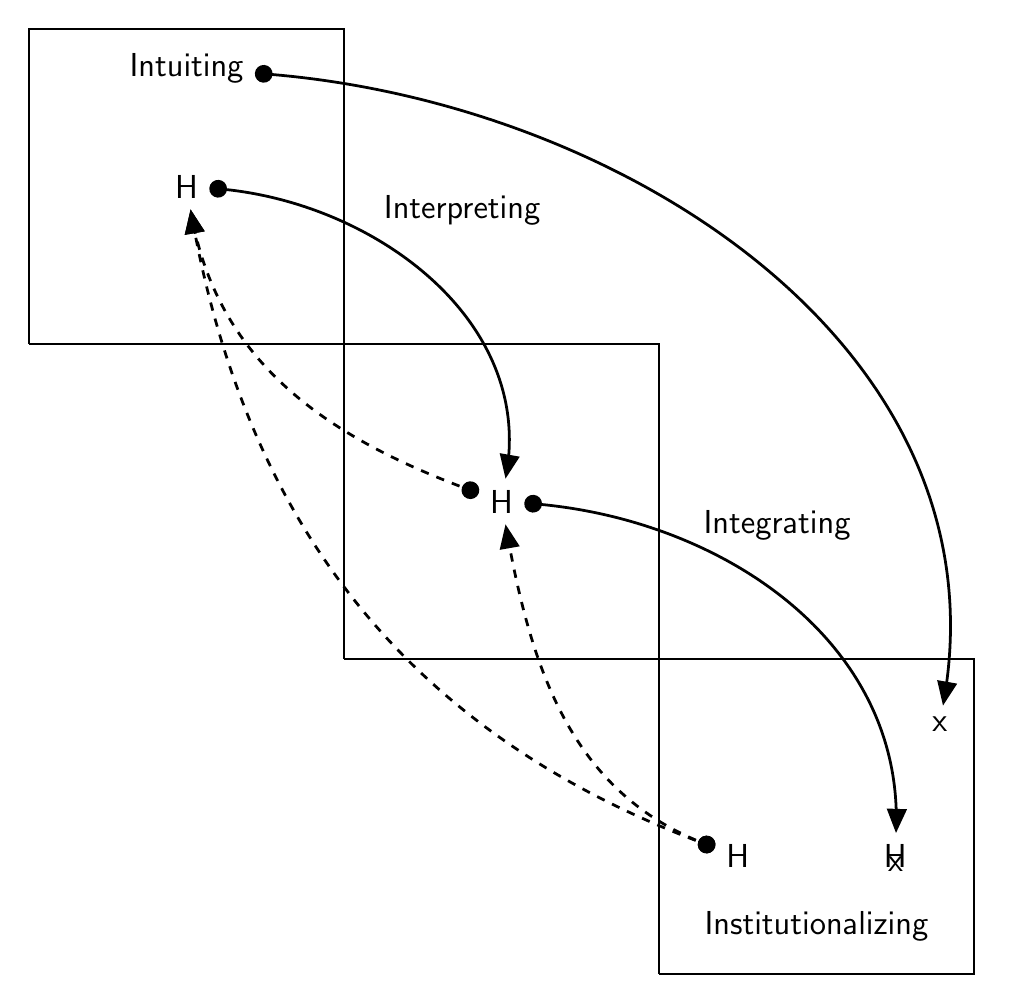
\begin{tikzpicture}
  %  \tikzset{>=latex}
    \tikzset{>=triangle 45}
  \large
  %\draw[step=1cm,gray,very thin] (0,-8) grid (14,4);

  \draw [line width=1pt](0,0) -- (4,0) -- (4,4) -- (0,4) -- (0,0);
\node (B1) at (2,2) {H};
\node (U) at (2,3.5) {Intuiting};
\node (R) at (5.5,1.7) {Interpreting};

\draw[line width=1pt] (4,-4) -- (8,-4) -- (8,0) -- (4,0) -- (4,-4);
\node (B2) at (6,-2) {H};
\node (G) at (9.5,-2.3) {Integrating};


\draw [line width=1pt](8,-8) -- (12,-8) -- (12,-4) -- (8,-4) -- (8,-8);
\node (B3R) at (11,-6.5) {H};
\node (B3L) at (9,-6.5) {H};

\node (Z) at (10, -7.4) {Institutionalizing};

\node[above=2cm of Z.north east] (RRZ){x};
\node[right=.01mm of Z, yshift=8mm,xshift=-8mm] (RZ){x};

\draw [*->,line width=1pt] (B1) to [out=-4,in=80] (B2);
\draw [*->,line width=1pt,dashed] (B2) to [out=160,in=280] (B1);


\draw [*->,line width=1pt] (U) to [out=-4,in=80] (RRZ);

\draw [*->,line width=1pt] (B2) to [out=-4,in=88] (B3R);

\draw [*->,line width=1pt, dashed] (B3L) to [out=160,in=280] (B2);
\draw [*->,line width=1pt, dashed] (B3L) to [out=160,in=280] (B1);


\end{tikzpicture}
\end{document}
